% %% %%%%%%%%%%%%%%%%%%%%%%%%%%%%%%%%%%%%%%%%%%%%%%%%%%%%%%%%%%
% objective.tex
%
% Author:  Mauricio Matamoros
% License: MIT
%
% %% %%%%%%%%%%%%%%%%%%%%%%%%%%%%%%%%%%%%%%%%%%%%%%%%%%%%%%%%%%

%!TEX root = ../main.tex
%!TEX root = ../references.bib

\subsection{Paso 1: Configuración del Simulador}%
\label{sec:step1}

Descargue el simulador de \url{https://github.com/kyordhel/RPiVirtualBoard} ejecutando la siguiente línea de comandos:

\begin{Verbatim}[fontsize=\footnotesize]
git clone https://github.com/kyordhel/RPiVirtualBoard.git
cd RPiVirtualBoard
\end{Verbatim}

A continuación instale todas las dependencias requeridas por el simulador usando \emph{pip}:

\begin{Verbatim}[fontsize=\footnotesize]
sudo apt install python3-tk
pip install --user -r requirements.txt
\end{Verbatim}

Finalmente, pruebe el simulador ejecutando la siguiente línea:

\begin{Verbatim}[fontsize=\footnotesize]
./blink.py
\end{Verbatim}

O bien, si desea mantener el simulador conmo un proyecto aislado y cuenta con la utilería \emph{pipenv}\footnotemark{} para tal propósito, después de clonar el proyecto basta con ejecutar:

\begin{Verbatim}[fontsize=\footnotesize]
pipenv run python blink.py
\end{Verbatim}

Si la configuración es correcta, verá una ventana similar a la de la \Cref{fig:simboard} con uno de los leds virtuales parpadeando.
Este simulador implementa el circuito mostrado en la \Cref{fig:wiring-diagram}

\begin{figure}[H]
	\centering%
	\begin{subfigure}{0.49\textwidth}
		\centering%
		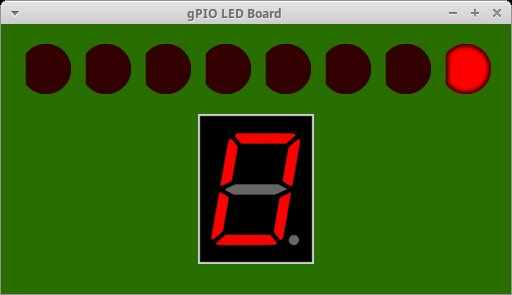
\includegraphics[width=0.9\textwidth,height=8cm,keepaspectratio]{img/simboard.jpg} %CHKTEX 8
		\caption{Simulador de tarjeta con leds para la GPIO de la Raspberry Pi}
		\label{fig:simboard} %CHKTEX 24
	\end{subfigure}
	\hfill
	\begin{subfigure}{0.49\textwidth}
		\centering%
		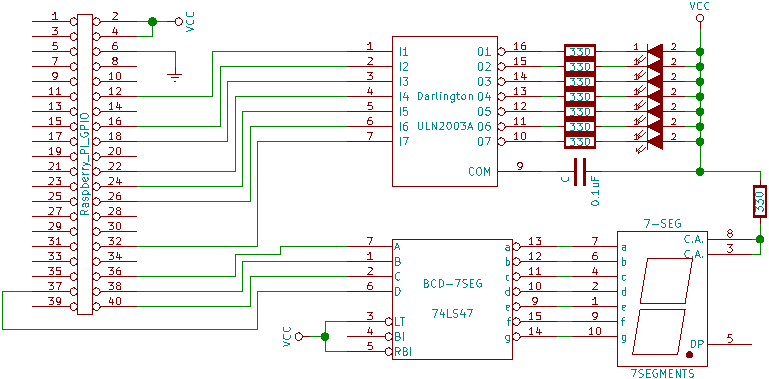
\includegraphics[width=0.9\columnwidth,height=8cm,keepaspectratio]{img/diagram.pdf} %CHKTEX 8
		\caption{Circuito implementado en el simulador}
		\label{fig:wiring-diagram} %CHKTEX 24
	\end{subfigure}
	\caption{Simulador y circuito implementado}
	\label{fig:sim} %CHKTEX 24
\end{figure}

\footnotetext{\emph{pipenv} es una herramienta que facilita la creación y administración de entornos virtuales en cualquier proyecto escritos en Python, llevando un control riguroso de los paquetes de los que depende dicho proyecto. Se puede instalar fácilmente con la línea \texttt{pip install --user pipenv}}
